\section{Supervision}

La supervision d'une infrastructure informatique consiste à vérifier à interval régulier la bonne santé des zones critiques pour en assurer la disponiblitité.
La supervision est un enjeux majeur d'une bonne infrastructure car elle permet d'être averti d'une panne des qu'elle se produit pour agire le plus rapidement possible.

Dans notre infrastructure composée de 2 serveurs et 5 machines virtuelle, nous avons choisi centreon comme superviseur.
Centreon est un système tout-en-un permettant de vérifier, à l'aide du protocol SNMP, la bonne santé des équipements.
Nous l'avons choisis pour sa facilité d'utilisation et pour sa propriété décentralisé.

Centreon met à disposition une architecture décentralisée permettant de gèrer un grand parc de machines.
Cette architecture est composée d'un serveur dit \emph{central} qui stock les données et dispose d'une interface d'administration web.
On trouve ensuite des serveurs dits \emph{Pollers} en charge de collecter les données des serveurs au travers de \emph{plugins}.

	\subsection{Installation}

	\subsubsection{Serveur central}

	Nous avons installé Centreon sur une nouvelle machine virtuelle.
	L'installation dispose alors de son propre serveur ce qui nous a permis d'utiliser le disque d'installation de base de Centreon.
	La procédure d'installation s'éfféctue comme suit :

	\begin{enumerate}
		\item Envoyer l'image ISO de centreon sur la machine ESXI
		\item Démarrer la machine virtuelle puis démarrer l'installation en choisissant le premier élément
		\item Suivre les étapes de l'installation en suivant les instructions suivantes
			\begin{itemize}
				\item Choisir la langue Française
				\item Prendre l'ensemble de l'espace disponible sur le disque virtuel
				\item Configurer le mot de passe root; Nous l'avons définis sur \texttt{Cesi2017!}
				\item Configurer le nom d'hote; Nous l'avons définis sur \texttt{Centreon-master}
			\end{itemize}
		\item Lors de la demande du type de serveur a installer, on choisis \texttt{Central server with database} pour disposer d'une base de données et de l'interface web
		\item Retirer l'image de la machine virtuelle
		\item Redémarrer le système
	\end{enumerate}

	L'installation faite, il suffit de se rendre, avec un navigateur, sur l'adresse du serveur Centreon pour poursuivre l'installation en ligne.

	\begin{enumerate}
		\item Se connecter en SSH au serveur Centreon
		\item Configurer le fuseau horaire PHP
		\begin{itemize}
			\item Dans le fichier \tetxttt{/etc/php.ini}
			\item Ligne \texttt{946}
			\item Décommenter la ligne \texttt{date.timezone = }
			\item Donner la valeur \texttt{date.timezone = Europe/Paris}
		\end{itemize}
		\item Redémarrer apache avec \texttt{service httpd restart}
		\item Retourner dans l'installation web
		\item On laissera les valeurs de chemins par défaut
		\item Configurer l'utilisateur administrateur, nous utiliserons ici les données de connexion suivantes
		\begin{description}
			\item[Login] admin
			\item[Password] \texttt{dcfvgbhn}
			\item[First Name] \texttt{Tanguy}
			\item[Last Name] \texttt{Blochet}
			\item[email] \texttt{tanguy.blochet@viacesi.fr}
		\end{description}
		\item Configurer le mot de passe de la base de données centreon; nous utiliserons \texttt{root}
		\item L'installation se poursuit avec la mise en place de la base de données
	\end{enumerate}

	Apres ces étapes, l'installation est complète et centreon pleinement fonctionnel

	\subsubsection{Installation du Poller}

	L'installation du poller s'éfféctue comme une installation du central.
	Mais lors du choix du type de serveur à installer, il faut choisir \texttt{Poller server}.
	De plus il n'y a pas d'installation Web à éfféctuer.

	\subsection{Configuration}

		\subsection{Plugins}

		Les plugins sont la base de la supervision, ils sont fournis par Centreon et se composent de multiples commandes linux permettant de faire des requètes normalisés pour controller la santé de l'infrastructure.

		\begin{enumerate}
			\item Sur la page \emph{Administration > Extentions}
			\item Activer l'extention \texttt{centreon-license-manager} et \texttt{centreon-pp-manager}.
			\item Sur la page \emph{Configuration > Plugin Pack}
			\item Installer les plugins \texttt{base-generic}, \texttt{Linux} et \texttt{Windows}
		\end{enumerate}

		Ces plugins composent la base du fonctionnement de Centreon.
		Ils donnent une base de commandes permettant de vérifier les systèmes sous différents angles.

		\subsection{Ajout d'une commande}

		Une commande est une référence, dans centreon, d'un programme présent sur le serveur permettant de vérifier la bonne santé d'une machine.

		Ces commandes utilisent les plugins centreon ou nagios interne ou installés a l'aide de plugins.

		\begin{enumerate}
			\item Aller dans la section \emph{Configuration > Commands}
			\item Ajouter une commande
			\item Donner un nom à la commande
			\item Donner le corps de la commande qui sera éxécuté dans l'evironnement du poller
		\end{enumerate}

		Il est possible d'ajouter des arguments dans le corps de la commande en utilisant la syntaxe \texttt{\$ARG1\$}.
		On peut alors donner un description des arguments dans la section \emph{Argument Descriptions}.

		Ces arguments seront demandés des l'utilisation de la commande et ils sont três utils pour définir des seuils ou des valeurs relatives.

		De plus, certains arguments sont prédéfinis et relatifs a l'hote ou au service.
		On les retrouve dans la zone à droite du corps de la commande lors de l'édition de celle-ci.

		\begin{figure}
			\begin{tabulary}{\textwidth}{|C|L|}
				\hline
				Commande & Description \\
				\hline
				\hline
				centreon\_linux\_snmp.pl --plugin=os::linux::snmp::plugin --mode=cpu & Permet le monitoring de la valeur du CPU sur les machines Linux\\
				\hline
				centreon\_linux\_snmp.pl --plugin=os::linux::snmp::plugin --mode=storage & Permet le monitoring du remplissage des disques sur les machines Linux\\
				\hline
				centreon\_linux\_snmp.pl --plugin=os::linux::snmp::plugin --mode=storage & Permet le monitoring du remplissage des disques sur les machines Linux\\
				\hline
				centreon\_linux\_snmp.pl --plugin=os::linux::snmp::plugin --mode=memory & Permet le monitoring de la mémoire RAM sur les machines Linux\\
				\hline
				centreon\_linux\_snmp.pl --plugin=os::linux::snmp::plugin --mode=interface & Permet le monitoring du traffic réseau sur les machines Linux\\
				\hline
				\hline
				centreon\_windows\_snmp.pl --plugin=os::windows::snmp::plugin --mode=cpu & Permet le monitoring de la valeur du CPU sur les machines Windows\\
				\hline
				centreon\_windows\_snmp.pl --plugin=os::windows::snmp::plugin --mode=storage & Permet le monitoring du remplissage des disques sur les machines Windows\\
				\hline
				centreon\_windows\_snmp.pl --plugin=os::windows::snmp::plugin --mode=storage & Permet le monitoring du remplissage des disques sur les machines Windows\\
				\hline
				centreon\_windows\_snmp.pl --plugin=os::windows::snmp::plugin --mode=memory & Permet le monitoring de la mémoire RAM sur les machines Windows\\
				\hline
				centreon\_windows\_snmp.pl --plugin=os::windows::snmp::plugin --mode=interface & Permet le monitoring du traffic réseau sur les machines Windows\\
				\hline
				\hline
				check\_dhcp & Permet de vérifier le fonctionnement du DHCP sur un hote\\
				\hline
				check\_dns & Permet de vérifier que le serveur DNS renvoie bien la bonne adresse IP sur un nom de domaine spécifique\\
				\hline

			\end{tabulary}
			\caption{Commandes utilisés pour le monitoring de l'infrastructure}
		\end{figure}

		\clearpage

		\subsection{Ajout d'un hote}

		Un hote représente, dans centreon, une machine sur le réseau.

		\begin{enumerate}
			\item Aller dans la section \emph{Configuration > Hosts}
			\item Ajouter un hote
			\item Ajouter le nom et l'alias représentant l'hote de manière unique
			\item Ajouter l'ip pour contacter la machine
			\item Renseigner la communauté SNMP et la version de SNMP utilisé
			\item Définir le poller à utiliser
			\item Choisir la commande permettant de vérifier que l'hote est présent dans la section \emph{Check Command}
			\item Choisir la fréquence et la periode a observer dans la section \emph{Scheduling Option}
		\end{enumerate}

		\subsection{Ajout d'un service}

		Les services sont des systèmes permettant de vérifier que tout ce que le serveur doit fournir est bien mis a disposition.
		Ils servent aussi à vérifier certaines valeurs comme le CPU, la RAM, etc.

		Les services utilisent les commandes et demandent leurs éxécution à interval réguler.
		Ces commandes permettent de définir un etat au service.

		\begin{description}
			\item[OK] Le service n'as rien à signaler
			\item[WARNING] Le service est en etat dangereux et demande une attention dans les plus bref délais
			\item[CRITICAL] Le service n'est plus disponible ou les meusures sont dans le rouge; le serveur demande une intervention immédiate
		\end{description}

		\begin{enumerate}
			\item Aller dans la section \emph{Configuration > Services}
			\item Ajouter un service et lui donner un nom
			\item Donner les hotes utilisant ce service
			\item Donner la commande à éxécuter dans la section \emph{Check command}
			\item Définir la periode de vérification dans la section \emph{Service Scheduling Options}
		\end{enumerate}

		\subsection{Ajout d'un poller}

		Apres l'installation d'un poller, il faut l'ajouter à notre serveur central pour qu'ils communiquent.

		\begin{enumerate}
			\item Installer un Poller suivant la procédure donnée précédement
			\item Depuis le serveur central, générer une clé pour l'utilisateur \texttt{centreon} avec les commandes \texttt{su - centreon} et \texttt{ssh-keygen}
			\item Copier la clé vers le serveur poller avec la commande \texttt{ssh-copy-id}
			\item Ajouter le poller dans la section web \emph{Configuration > Poller}
			\item Ajouter un recuperateur de données en utilisant l'assistant dans \texttt{Configuration > Poller}
			\item Ajouter au moin un hote au poller dans les paramètres du poller
		\end{enumerate}


		\subsection{Monitoring}

		Le monitoring des services et hotes passent par la section \emph{Monitoring > Services}.
		Dans cette section on retrouve tout les services associés aux hotes et leurs status.

		Une page plus réduite et synthétique peut être trouvée dans la section \emph{Monitoring > Services Grid}

		\begin{figure}[h]
			\centering
			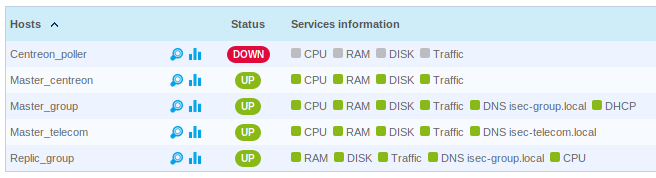
\includegraphics[scale=0.5]{Supervision/service-grid.png}
			\caption{Exemple d'hotes et de services sur l"interface de centreon}
		\end{figure}

		\subsubsection{Reporting}

		Le reporting est une fonctionnalité importante de centreon permettant de meusurer son SLA pour chaque Hote.

		Pour calculer le reporting, il faut, au préalable, éxécuter les commandes suivantes permettant de calculer le reporting pour la journée.

		\begin{lstlisting}[caption=Commandes permettant de calculer le reporting pour la journée en cours]
/usr/share/centreon/cron/eventReportBuilder
/usr/share/centreon/cron/dashboardBuilder
		\end{lstlisting}

		On retrouve alors les données du reporting dans la section \emph{Reporting > Dashboard} sur l'interface WEB.

		Il est conseillé de mettre ces commandes dans la table cron pour l'éxécuter chaque jour.

		\begin{figure}[h]
			\centering
			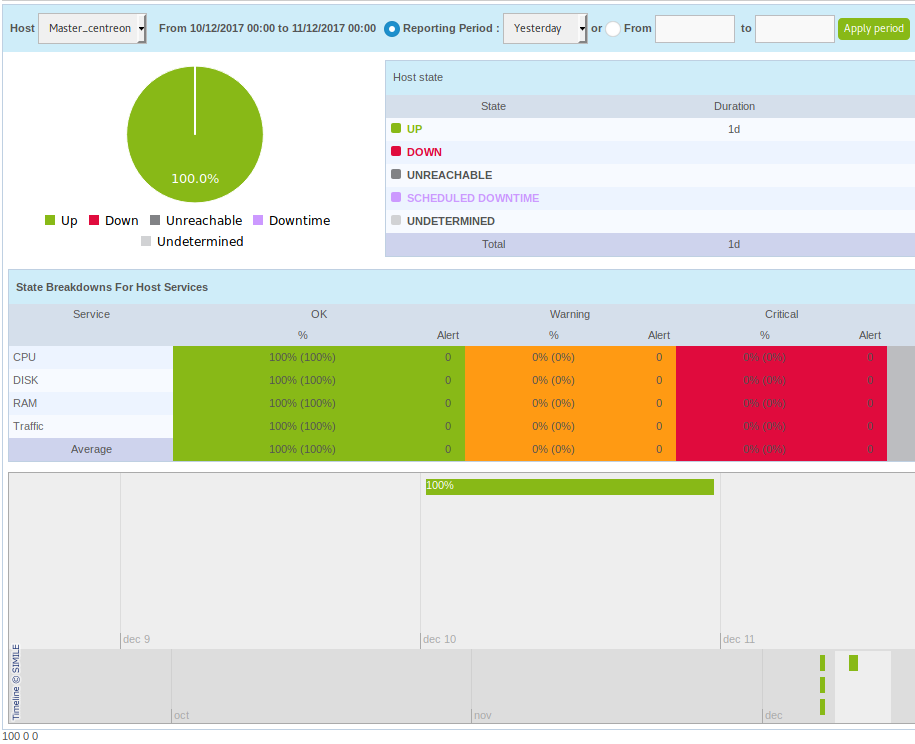
\includegraphics[scale=0.5]{Supervision/monitoring.png}
			\caption{Exemple d'interface de reporting}
		\end{figure}

	\subsection{Sauvegarde}

	Pour garantire une réinstallation possible, nous avons créé un script permettant d'enregistrer un sauvegarde de la configuration de Centreon.
	Ce script sauvegarde les fichiers de configuration et les plugins dans des archives TAR.
	Il s'occupe aussi de sauvegarder la base de données.

	Ce script va de paire avec le script de restauration éfféctuant les oppérations inverses pour restaurer les configurations, plugins et bases de données.

	\paragraph{Attention} Vérifiez bien que la version de Centréon utilisé pour la restauration est la même que celle utilisée pour la sauvegarde. Les bases de données sont, le plus souvent, incompatibles.
